\documentclass[tikz]{standalone}

\usepackage[T1]{fontenc}
\usepackage[english]{babel}

\usepackage{standalone}

\usepackage{pgfplots}

\usepackage{tikz}
\usetikzlibrary{calc, 3d}

\begin{document}
    \begin{tikzpicture}
    	\node (residual) at (0,0) {
            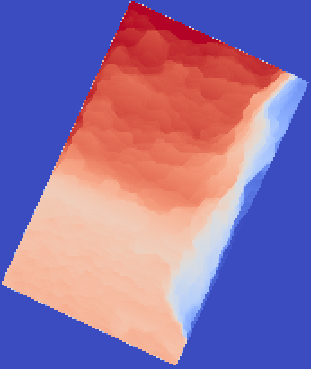
\includegraphics[height=1cm, angle=270]{images/introduction/graphical_abstract/residual}
        };
        \path (residual.south) node[anchor=north] (residual_legend) {\tiny (c) Height-based};
        
        \path (residual.west) + (-.4,0) node[anchor=east] (facet_graph) {\includestandalone[mode=buildmissing, height=1cm]{figures/graphical_abstract/building_graph}};
        \path (facet_graph |- residual_legend) node (facet_graph_legend) {\tiny (b) Geometric};

        \path (facet_graph.west) + (-1,0) node[anchor=east] (model) {\includestandalone[mode=buildmissing, height=1cm]{figures/graphical_abstract/building_model}};
        \path (model |- residual_legend) node (model_legend) {\tiny (a) Input model};
        
        \path (residual.east) + (.8,0) node[anchor=west] (ortho_projection) {
            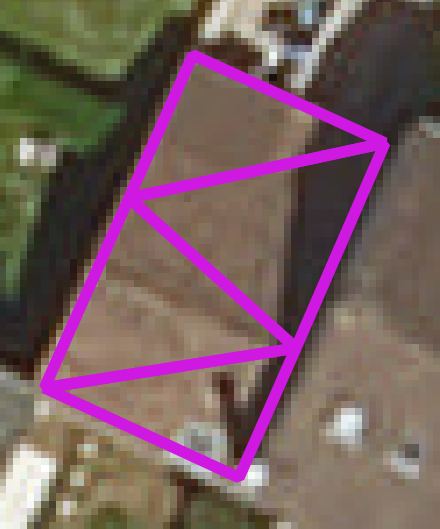
\includegraphics[height=1cm, angle=270]{images/introduction/graphical_abstract/orthoprojection}
        };
        \path (ortho_projection |- residual_legend) node (orthoprojection_legend) {\tiny (d) Image-based};
        
        \draw[decorate, decoration={brace, amplitude=3pt}] (orthoprojection_legend.south east) -- (facet_graph_legend.south west) node[midway, yshift=-8pt]{\tiny Features};

		\path (orthoprojection_legend.east |- ortho_projection) + (1,0) node[anchor=west] (errors) {\includestandalone[mode=buildmissing, height=1cm]{figures/graphical_abstract/building_errors}};
        \path (errors |- residual_legend) node (errors_legend) {\tiny (e) Erroneous building};
        \path (errors_legend.east |- errors.north) node[align=left, anchor=south east] (errors_list) {\tiny {\color{blue}\(\blacksquare\) Modeling error}};
        \path (errors_list.north east) node[align=left, anchor=east] (errors_list) {\tiny {\color{red}\(\blacksquare\) Fidelity error}};
        
        \path[draw, ->, line width=1pt, rounded corners=10pt, green] (model_legend.east |- model) -- (facet_graph.west);
        \path[draw, ->, line width=1pt, rounded corners=10pt, green] (orthoprojection_legend.east |- ortho_projection) -- (errors);
    \end{tikzpicture}
\end{document}
